\documentclass[11pt,a4paper]{article}
\usepackage[utf8]{inputenc}
\usepackage[T1]{fontenc}
\usepackage{lmodern}
\usepackage[spanish]{babel}
\usepackage{geometry}
\geometry{left=2.5cm, right=2.5cm, top=3cm, bottom=3cm}
\usepackage{titlesec}
\usepackage{parskip}
\usepackage{xcolor}
\usepackage{fancyhdr}
\usepackage{hyperref}
\usepackage{graphicx} % Added for image support

% Colors
\definecolor{primary}{RGB}{44, 62, 80}
\definecolor{accent}{RGB}{192, 57, 43}

% Formatting
\titleformat{\section}{\color{primary}\Large\bfseries}{\thesection}{1em}{}[\vspace{-0.5ex}\rule{\textwidth}{1pt}]
\titleformat{\subsection}{\color{accent}\large\bfseries}{\thesubsection}{1em}{}

% Header and Footer
\pagestyle{fancy}
\fancyhf{}
\fancyhead[L]{\textbf{High Concept Document}}
\fancyhead[R]{BombaStudios SL}
\fancyfoot[C]{\thepage}

\begin{document}

\begin{titlepage}
    \centering
    \vspace*{1cm}
    {\Huge \textbf{\textcolor{primary}{La Torre de Ceniza}}}\\[1cm]
    
    % Included the vertical image here, constrained by height so it fits well on the title page
    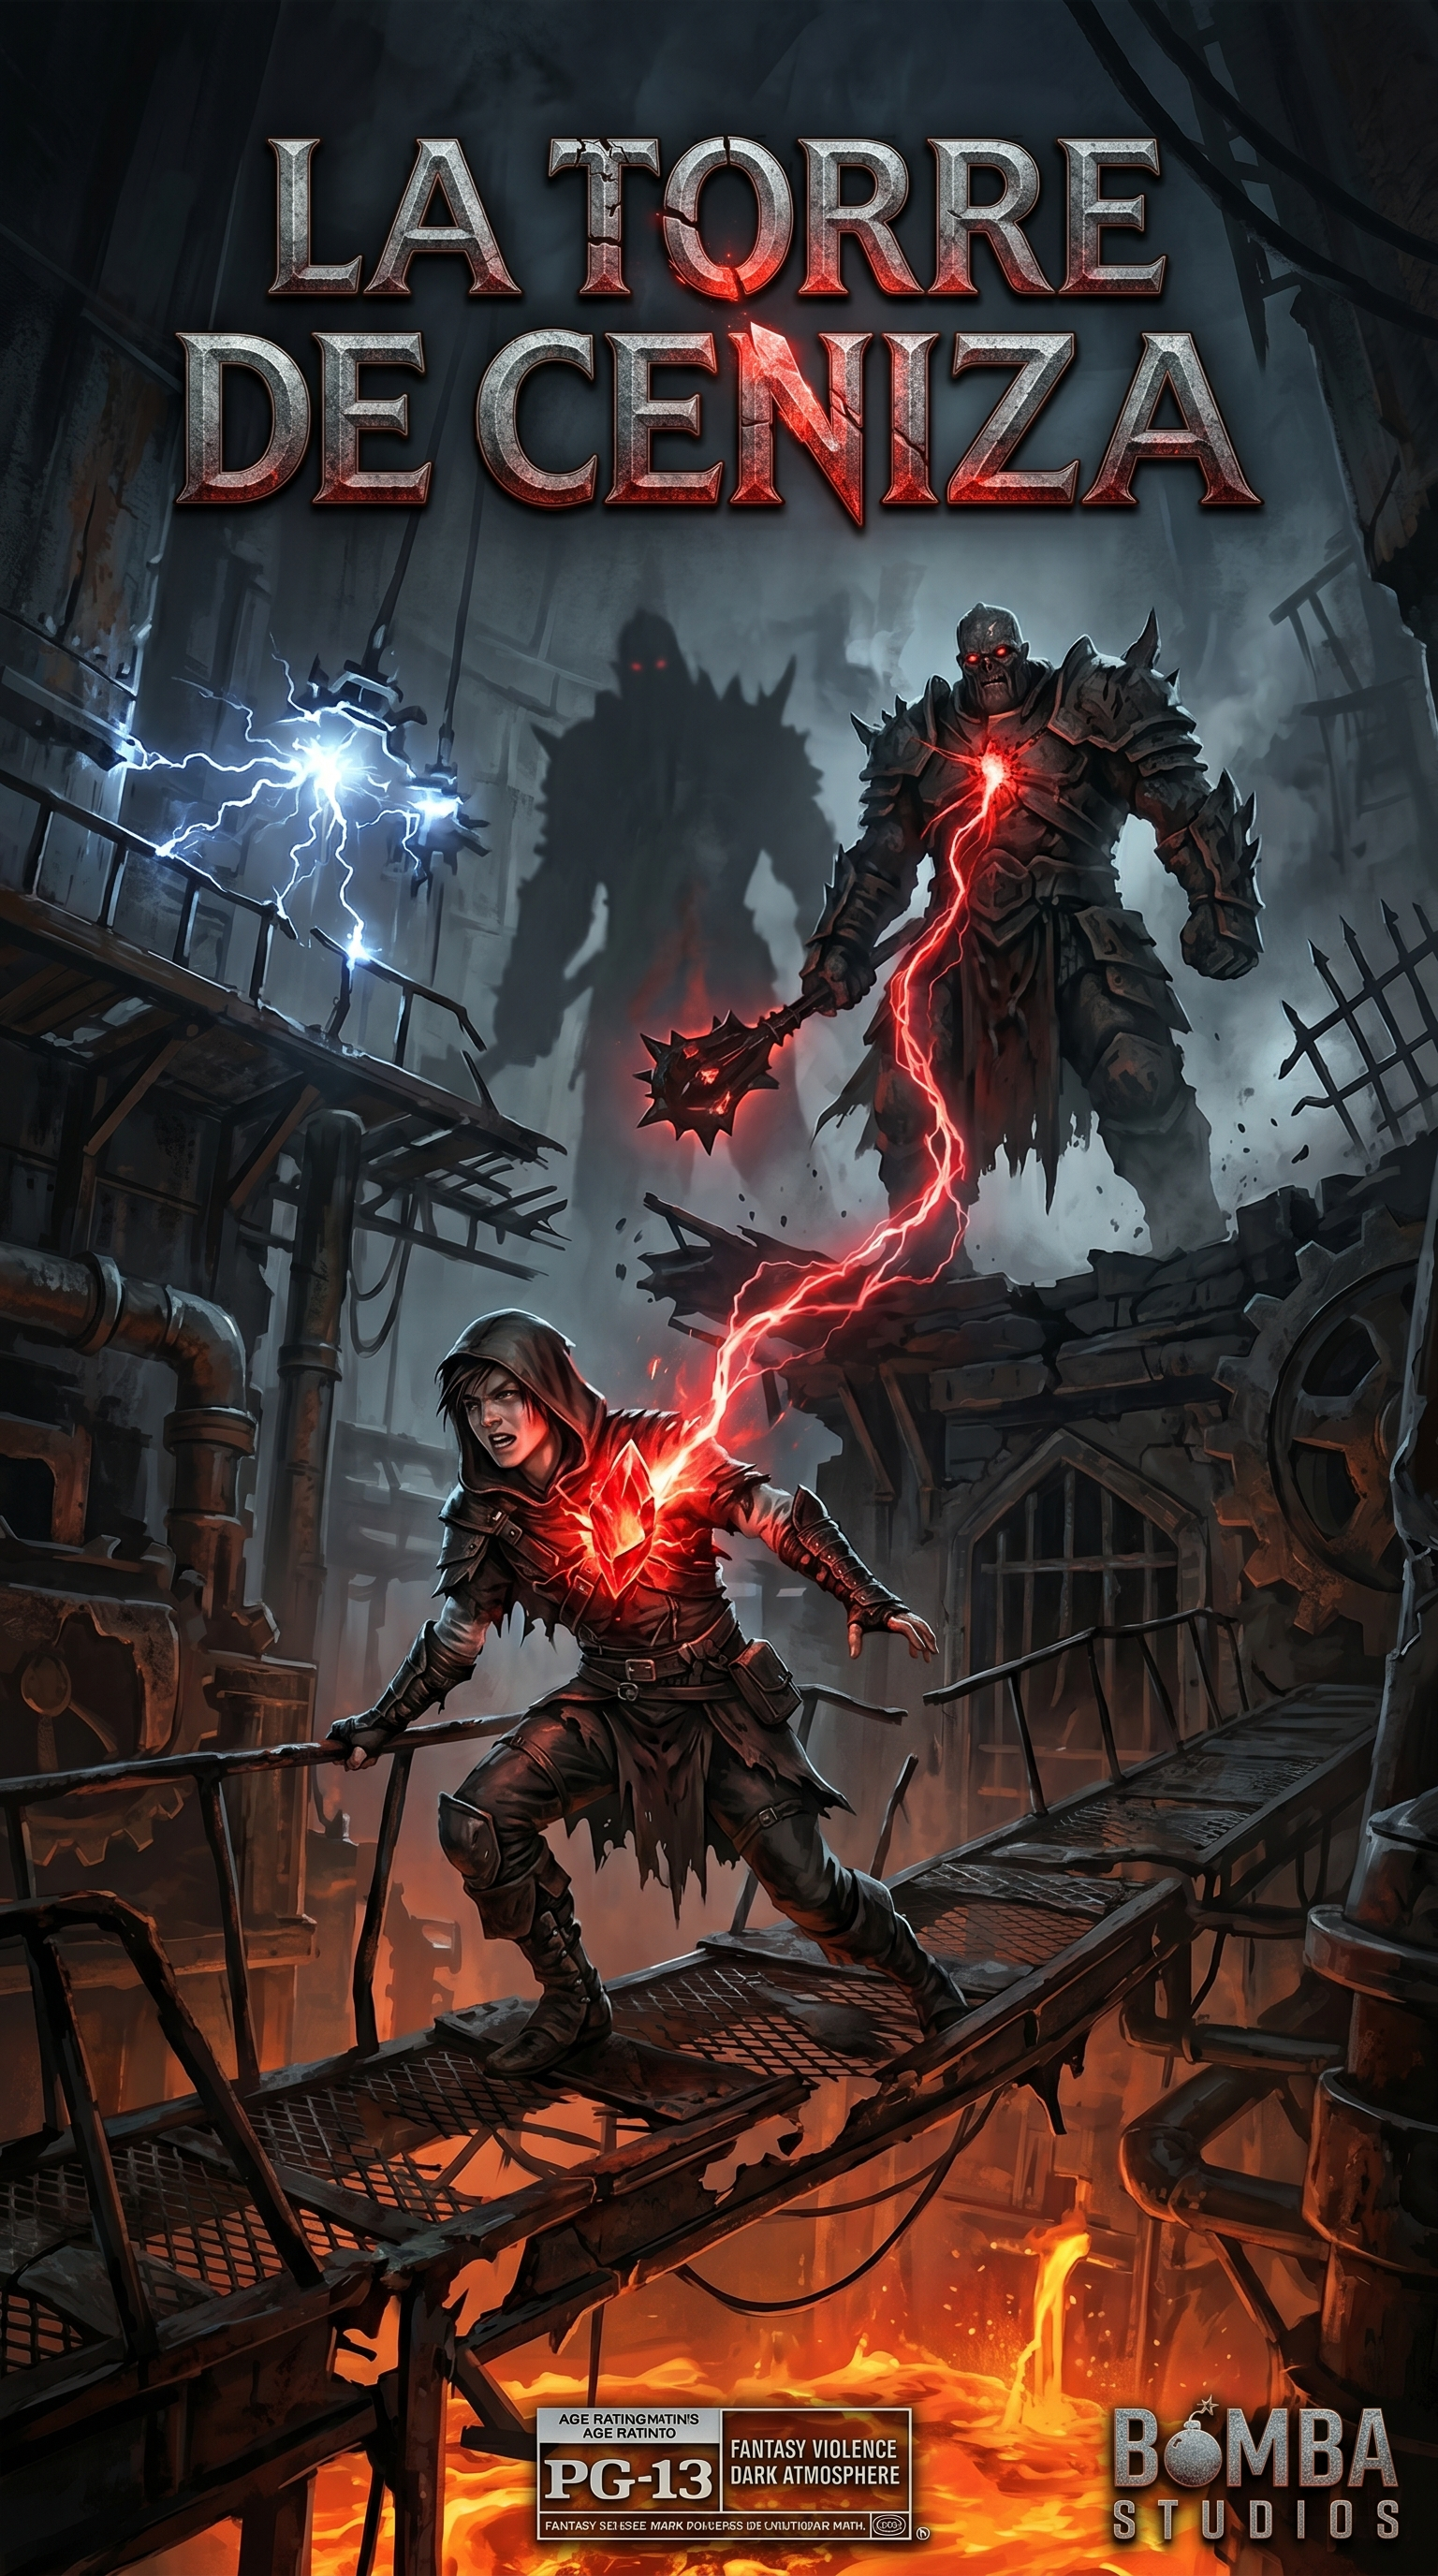
\includegraphics[height=11cm, keepaspectratio]{Arte.png}\\[1cm]
    
    {\LARGE \textbf{High Concept Document}}\\[1cm]
    {\Large \textbf{BombaStudios SL}}\\[0.5cm]
    \vfill
    \textbf{Equipo:}\\[0.5cm]
    \textbf{Antonio} -- Programador, Interfaz\\
    \textbf{Abdullah} -- Diseñador, Programador\\[1cm]
\end{titlepage}

\newpage

\section*{Idea / Narrativa}

\subsection*{La Premisa (``La muerte no es el final'')}
El juego le da la vuelta a los combates tradicionales contra jefes. Controlas a un personaje ágil pero frágil que no puede hacerle ningún daño a su enemigo con ataques normales. La única forma de ganar es el sacrificio: debes usar las trampas del escenario para acabar con tu propia vida y, al hacerlo, destruir al monstruo que está mágicamente conectado a ti.

\subsection*{La Historia: El Ciclo de Ceniza}
Vesper es un joven ladrón que entra en la Torre de Ceniza para robar el Núcleo Carmesí. Al intentar cogerlo, el cristal estalla. Una mitad se clava en su pecho y la otra despierta a Malikor, un gigante implacable. 

Debido al poder del fragmento en su pecho, Vesper está atrapado en un bucle; si Malikor lo aplasta, el cristal lo reconstruye. Pero cada resurrección agrieta más la gema. Si se rompe del todo, el alma de Vesper desaparecerá para siempre.

\subsection*{El Objetivo: Romper el Vínculo}
Como sus vidas están unidas por el cristal, Vesper entiende que dejarse matar a golpes no sirve de nada, solo alarga la tortura. Para romper este ciclo de muertes infinitas y ganar, Vesper debe sobrevivir a la persecución, atraer a Malikor hacia puntos estratégicos de la torre y aprovechar elementos peligrosos del entorno para hacerle daño. Esa enorme energía sobrecargará el vínculo mágico, causando una explosión final que destruirá el cristal, acabando con ambos para siempre.

\section*{Tipo de Juego}
2D. Vista lateral (plataformas) en un mapa vertical, centrado en una única arena de combate.

\section*{Ambientación}
La ambientación se define como Claustrofobia Industrial y Fantasía Decadente. El entorno no es un simple decorado, sino un lugar hostil que hace sentir al jugador que está atrapado y que el sacrificio es su única salida. Se basa en tres puntos clave:

\subsection*{Colores y Claridad Visual}
\begin{itemize}
    \item \textbf{El Fondo:} Colores fríos y apagados que dan la sensación de una fábrica antigua y abandonada.
    \item \textbf{La Acción:} El jugador, el jefe, el vínculo mágico y las trampas deben tener colores brillantes y llamativos. Este contraste permite ver al instante dónde está el peligro durante la persecución.
\end{itemize}

\subsection*{Sonido y Tensión}
\begin{itemize}
    \item \textbf{Fondo:} Un zumbido grave de máquinas apagadas y crujidos del metal.
    \item \textbf{El Jefe:} La presencia de Malikor se nota por sus pasos: golpes metálicos lentos y pesados que hacen temblar un poco la pantalla.
    \item \textbf{Las Trampas:} Arriba, el chisporroteo inestable de la electricidad; abajo, el sonido espeso de la lava burbujeante.
\end{itemize}

\subsection*{La Historia del Escenario}
El nivel debe mostrar a simple vista que esta Torre fue una prisión que fracasó. Las plataformas metálicas están abolladas y las rejas rotas por golpes antiguos. Las luces de las trampas eléctricas parpadean, proyectando sombras alargadas de Malikor en las paredes para que parezca aún más gigantesco e intimidante.

\section*{Mecánicas}

\subsection*{1. Plataformeo y Evasión}
Vesper tiene controles ágiles orientados a la huida:
\begin{itemize}
    \item Movimiento lateral (izquierda/derecha)
    \item Salto
    \item Doble salto
\end{itemize}

\subsection*{2. Inmunidad del Enemigo}
Cualquier intento de golpear o disparar al jefe no le restará salud; es completamente invulnerable. Malikor te seguirá de forma constante por la arena. Esto fuerza al jugador a entender rápidamente que la solución para ganar está en usar el entorno, no en pelear.

\subsection*{3. Resurrección Limitada}
Si Malikor te alcanza y te golpea, mueres. Sin embargo, gracias al cristal mágico, revives casi al instante para seguir huyendo. Esto consume una ``vida''. Tienes un número limitado de resurrecciones. Si agotas todas tus oportunidades sin lograr tu objetivo, pierdes la partida (Game Over).

\subsection*{4. El Sacrificio}
Para ganar, el jugador debe usar las trampas extremas del nivel de forma estratégica. Tienes que atraer a Malikor hacia la electricidad (arriba) o la lava (abajo). Cuando el jefe esté muy cerca de ti, debes lanzarte voluntariamente a la trampa mortal. Tras varias muertes voluntarias usando las trampas del escenario, el vínculo mágico explota, destruyéndolo y desafortunadamente, acabando finalmente con la vida de Vesper.

\section*{Objetivo}
El objetivo principal del jugador es romper el bucle mágico y destruir a Malikor, el jefe invulnerable de la Torre de Ceniza. En esencia, derrotar al boss utilizando estratégicamente distintos tipos de muerte, aprendiendo cuáles son más eficaces y optimizando cada intento hasta vaciar su barra de vida.

\section*{Relación con el Tema de la Jam}
El juego se basa directamente en este concepto, transformando la muerte en la mecánica principal de progreso. En lugar de ser una penalización, morir es la única forma de avanzar y derrotar al enemigo. Cada muerte aporta valor y acerca al jugador a la victoria, reforzando la idea de que el final no está en fallar, sino en dejar de intentarlo.

\end{document}
